% ==========================================================================
\section{A playbook for a timed exam}
\label{sec:exam}

Under time pressure the value of a diagram is not elegance; it is that it removes
bookkeeping. The protocol below is four steps and takes about fifteen seconds per
exercise.

\begin{recipe}[The four steps]
\begin{enumerate}[leftmargin=1.6em,itemsep=1pt]
\item \textbf{Classify.} Is the task about (i) a \emph{solution set}, (ii) a
  \emph{composition or inverse}, (iii) a \emph{quantity to bound}, or (iv) a
  \emph{computation}?
\item \textbf{Pick the language.} (i) number line / sign line; (ii) commutative or
  bag-and-arrow diagram, or the mirror $y=x$; (iii) triangle, chain, or a Nelsen figure;
  (iv) no diagram -- compute, but sketch the expected answer first to catch sign errors.
\item \textbf{Draw the canonical picture} large enough to write on, and mark every
  endpoint, branch and case that the picture forces you to consider.
\item \textbf{Write the residue}, one line, next to the drawing. This is what converts a
  drawing into an accepted proof.
\end{enumerate}
\end{recipe}

\subsection{Four model answers}

\begin{figure}[H]
\centering
\begin{tikzpicture}[x=0.36cm,y=1cm]
  \draw[axis] (-11,0) -- (7,0);
  \fill[blue!20] (-9,-0.13) rectangle (-7,0.13);
  \fill[blue!20] (3,-0.13) rectangle (5,0.13);
  \draw[very thick,blue!60!black] (-9,0) -- (-7,0);
  \draw[very thick,blue!60!black] (3,0) -- (5,0);
  \foreach \p in {-9,-7,-2,3,5}{\draw (\p,-0.13) -- (\p,0.13);}
  \foreach \p/\l in {-9/{-9},-7/{-7},-2/{-2},3/{3},5/{5}}
    {\node[font=\scriptsize,below=3pt] at (\p,-0.1) {$\l$};}
  \foreach \p in {-9,-7,3,5}{\draw[fill=white,thick] (\p,0) circle (2pt);}
  \node[font=\scriptsize,anchor=west] at (5.6,0.55)
     {$|x+2|\in(5,7)$, both branches};
\end{tikzpicture}
\caption*{\textbf{(a) Solve $\bigl||x+2|-6\bigr|<1$ (1.12 b).} \emph{Write:}
``$|x+2|-6\in(-1,1)\Rightarrow|x+2|\in(5,7)\Rightarrow x+2\in(5,7)\cup(-7,-5)$'', then
the drawing, then the answer $x\in(-9,-7)\cup(3,5)$. Total: two lines and one line
segment. The picture's job is to stop you dropping the negative branch.}
\end{figure}

\begin{figure}[H]
\centering
\begin{tikzpicture}[x=0.95cm,y=0.95cm]
  \clip (-2.9,-2.9) rectangle (2.9,2.9);
  \draw[axis] (-2.8,0) -- (2.8,0);
  \draw[axis] (0,-2.8) -- (0,2.8);
  \draw[gray,dashed] (-2.7,-2.7) -- (2.7,2.7);
  \draw[very thick,blue!60!black,domain=-2.8:-0.85,samples=40,smooth]
     plot (\x,{(2*\x-1)/(3*\x+2)});
  \draw[very thick,blue!60!black,domain=-0.45:2.8,samples=40,smooth]
     plot (\x,{(2*\x-1)/(3*\x+2)});
  \draw[very thick,red!60!black,domain=-2.8:0.4,samples=40,smooth]
     plot (\x,{(-2*\x-1)/(3*\x-2)});
  \draw[very thick,red!60!black,domain=0.9:2.8,samples=40,smooth]
     plot (\x,{(-2*\x-1)/(3*\x-2)});
\end{tikzpicture}
\caption*{\textbf{(b) Invert $a(x)=\frac{2x-1}{3x+2}$ (2.3 a).} \emph{Write:} ``$y(3x+2)
=2x-1\Rightarrow x=\frac{-2y-1}{3y-2}$'', then draw the two curves and the mirror. The
drawing is the \emph{check}: if the red curve is not the mirror image of the blue one, the
algebra is wrong. Checking by picture is far faster than substituting back, and it
verifies \emph{both} triangles of Figure~\ref{fig:invunique} at once.}
\end{figure}

\begin{figure}[H]
\centering
\begin{tikzpicture}[x=1cm,y=1cm]
  \coordinate (P0) at (0,0);
  \coordinate (P1) at (1.5,0.9);
  \coordinate (P2) at (2.4,-0.1);
  \coordinate (P3) at (4.1,0.6);
  \coordinate (P4) at (5.2,-0.4);
  \draw[vec,blue!60!black] (P0) -- (P1);
  \draw[vec,blue!60!black] (P1) -- (P2);
  \draw[vec,blue!60!black] (P2) -- (P3);
  \draw[vec,blue!60!black] (P3) -- (P4);
  \draw[vec,dashed] (P0) -- (P4);
  \foreach \p in {P0,P1,P2,P3,P4} {\fill (\p) circle (1.5pt);}
  \node[font=\scriptsize,anchor=south] at (2.7,-0.75) {$\bigl|\sum a_i\bigr|$};
  \node[font=\scriptsize,anchor=south] at (0.6,0.5) {$|a_1|$};
\end{tikzpicture}
\caption*{\textbf{(c) Prove $|a_1+\dots+a_n|\le|a_1|+\dots+|a_n|$ (1.13).} \emph{Write:}
``induction; the step is the two-term case, which is the case distinction
$\operatorname{sign}a=\operatorname{sign}b$'' -- then the broken-line drawing. Marking
$n=2$ on the picture and saying ``iterate'' is the whole proof; graders accept it because
the induction is visible in the figure.}
\end{figure}

\begin{figure}[H]
\centering
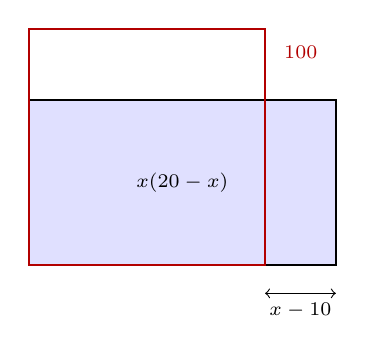
\begin{tikzpicture}[x=0.3cm,y=0.3cm]
  \draw[thick,fill=blue!12] (0,0) rectangle (13,7);
  \draw[thick,red!70!black] (0,0) rectangle (10,10);
  \node[font=\scriptsize] at (6.5,3.5) {$x(20-x)$};
  \node[font=\scriptsize,red!70!black,anchor=west] at (10.4,9) {$100$};
  \draw[<->] (10,-1.2) -- (13,-1.2) node[midway,below,font=\scriptsize]{$x-10$};
\end{tikzpicture}
\caption*{\textbf{(d) Split $20$ for maximal product (4.11 a).} \emph{Write:}
``$x(20-x)=100-(x-10)^{2}$'', then the drawing. One line of algebra, one square, and the
maximum $100$ at $x=10$ is established -- faster and safer than differentiating.}
\end{figure}

\subsection{Time budget for a 90-minute paper}

\begin{center}
\small
\begin{tabular}{@{}p{4.6cm}p{2.4cm}p{7.4cm}@{}}
\toprule
Task type & Budget & What goes on the paper \\
\midrule
Inequality, solution set & 3--4 min & sign line or interval picture $+$ answer with
  endpoint status \\
Inverse / composite & 4--5 min & the algebra, then the mirror picture as a check \\
Injectivity, surjectivity & 2 min & bag picture or one monotonicity line \\
Estimate, triangle inequality & 4 min & the chain drawing $+$ the case distinction \\
Limit, $\varepsilon$--$\delta$ & 6--8 min & band/strip picture $+$ the $\delta$ formula \\
Curve discussion & 12--15 min & two sign rows, then one careful graph \\
Optimisation & 6--8 min & the superposition picture $+$ the completed square \\
Symbolic computation & rest & no picture, but sketch the expected answer first \\
\bottomrule
\end{tabular}
\end{center}

\subsection{Turning a picture into accepted prose in one sentence}

Each language has a standard verbal rendering. Memorise these and you can always convert.

\begin{center}
\small
\begin{tabular}{@{}p{4.6cm}p{9.8cm}@{}}
\toprule
Picture & Sentence \\
\midrule
Two triangles closing & ``Both composites are the identity, hence $g=f^{-1}$.'' \\
Chain of arrows & ``By the triangle inequality applied $n-1$ times \dots'' \\
Nested discs & ``If $\dd(x,y)<r$ then the ball of radius $r-\dd(x,y)$ about $y$ lies in
  the ball of radius $r$ about $x$.'' \\
Sign line & ``The product changes sign exactly at the roots; testing one point per
  interval gives \dots'' \\
Mirror in $y=x$ & ``$(a,b)$ is on the graph of $f$ iff $(b,a)$ is on the graph of
  $f^{-1}$.'' \\
Band and strip & ``For every $\varepsilon>0$ choose $\delta=\dots$; then
  $|x-c|<\delta$ implies $|f(x)-L|<\varepsilon$.'' \\
Bags and arrows & ``Distinct inputs have distinct images, and every output is hit.'' \\
Superposed figures & ``The difference of the two areas is a square, hence non-negative.''\\
\bottomrule
\end{tabular}
\end{center}

\subsection{The five traps, in the order in which they cost marks}

\begin{enumerate}[leftmargin=1.6em,itemsep=2pt]
\item \textbf{Endpoints.} A shaded interval does not record whether its ends belong to
  it. Draw filled/open circles \emph{as you shade}.
\item \textbf{A missing branch.} Every fold ($|\cdot|$, squaring, $\cos$) has two
  preimages; every square root has a sign condition. Count the branches in the picture
  before reading the answer.
\item \textbf{Domains.} A composite is only defined where the inner function lands in the
  domain of the outer one (exercise 2.10). Two graphs on one sheet hide this; write the
  domain next to the arrow.
\item \textbf{Non-generic configuration.} A drawing shows one case. If the statement has
  a parameter, ask which pictures the parameter can produce, and draw the extreme ones.
\item \textbf{Infinite processes.} A dissection can exhaust a region only in the limit
  (Figure~\ref{fig:geom}). A picture of infinitely many steps proves a statement about
  partial sums, never about the limit; the limit is always the residue.
\end{enumerate}

\subsection{Closing: the same two pictures, once more}

\begin{figure}[H]
\centering
\begin{tikzcd}[column sep=large,row sep=large]
\textbf{Kalkulus I} \arrow[r,"\text{same theorem}"] \arrow[d,"|x-y|"'] &
  \textbf{Line\'aris algebra I} \arrow[d,"\norm{u-v}"] \\
\text{triangle inequality} \arrow[r,leftrightarrow] & \text{triangle inequality} \\
\text{inverse function} \arrow[r,leftrightarrow] \arrow[u,"\text{composition}"] &
  \text{inverse matrix} \arrow[u,"\text{composition}"']
\end{tikzcd}
\caption{The whole document in one commutative diagram. The horizontal arrows are the two
overlaps; the vertical arrows say that both are statements about \emph{composition} -- in
a category enriched over $([0,\infty),\ge,+)$ for the triangle inequality, in an ordinary
category for the inverse. Formalised in
\lean{RequestProject/TriangleOverlap.lean} and \lean{RequestProject/InverseOverlap.lean};
the pictures of this document are certified in \lean{RequestProject/DiagramProofs.lean}.}
\label{fig:final}
\end{figure}

\section*{Sources and further reading}
\addcontentsline{toc}{section}{Sources and further reading}

\begin{itemize}\itemsep2pt
\item R.\ B.\ Nelsen, \emph{Proofs Without Words} (MAA) -- the standard collection of
  dissection and superposition arguments, including the semicircle picture for AM--GM and
  the staircase pictures for $\sum i$ and $\sum i^{2}$.
\item P.\ Soboci\'nski et al., \emph{Graphical Linear Algebra},
  \url{https://graphicallinearalgebra.net/} -- the string-diagram development of linear
  algebra used in Section~\ref{sec:string}.
\item F.\ W.\ Lawvere, \emph{Metric spaces, generalized logic, and closed categories}
  (1973) -- metric spaces as enriched categories; the source of
  Figure~\ref{fig:lawvere}.
\item A.\ Joyal and R.\ Street, \emph{The geometry of tensor calculus} -- the soundness
  and completeness theorem that makes string diagrams a proof system.
\item C.\ S.\ Peirce, \emph{Existential Graphs} -- the first complete diagrammatic
  calculus for logic (Figure~\ref{fig:peirce}).
\item The two course descriptions (\emph{Kalkulus I}, MBLK37E; \emph{Line\'aris algebra
  I}, MBLK15E) and the exercise sheet \lean{kalkulus\_gyakorlo.pdf} supplied with this
  project.
\end{itemize}
